\documentclass[a4paper]{scrartcl}

\usepackage[utf8]{inputenc}
%\usepackage[USenglish]{babel}
\usepackage{csquotes}

%More margins for annotations
%\usepackage[a4paper, top=2.5cm, bottom=2.5cm, left=2.5cm, right=2.5cm]{geometry}
\usepackage[a4paper, top=3.5cm, bottom=3.5cm, left=3.5cm, right=3.5cm]{geometry}

\usepackage[plainpages=false,pdfpagelabels,hidelinks,unicode]{hyperref}

\usepackage{amsmath}
\usepackage{amsfonts}

\usepackage{graphicx}
\usepackage{subcaption}

% math packages
\usepackage{amsmath}
\numberwithin{equation}{section}
\allowdisplaybreaks
\usepackage{amssymb}
\usepackage{commath}
\usepackage{mathtools}
\usepackage{bbm}
\usepackage{nicefrac}

\usepackage{siunitx}

\usepackage{amsthm}
\theoremstyle{plain}
  \newtheorem{theorem}{Theorem}
  \newtheorem{lemma}[theorem]{Lemma}
  \newtheorem{corollary}[theorem]{Corollary}
  \newtheorem{proposition}[theorem]{Proposition}
\theoremstyle{definition}
  \newtheorem{definition}[theorem]{Definition}
  \newtheorem{remark}[theorem]{Remark}
  \newtheorem{example}[theorem]{Example}
\numberwithin{theorem}{section}

% definitions
\newcommand{\N}{\mathbb{N}}
\newcommand{\R}{\mathbb{R}}
\newcommand{\CN}{\mathbb{C}}
\renewcommand{\H}{\mathcal{H}}
\renewcommand{\O}{\mathcal{O}}
\newcommand{\dt}{{\Delta t}}
\newcommand{\1}{\mathbbm{1}}
\newcommand{\e}{\mathrm{e}}
\newcommand{\scp}[2]{\left\langle{#1,\, #2}\right\rangle}
\newcommand{\I}{\operatorname{I}}
\newcommand{\lot}{\ell_{\mathrm{ot}}}

%tikz
\usepackage{tikz}
\usetikzlibrary{shapes.geometric, arrows}
\usetikzlibrary{calc}
\usepackage{color}

% LP-Box
\newcommand{\LPblock}[1]{
\tikzstyle{textbox} = [draw=black, fill=white, very thick,
    rectangle, rounded corners, inner sep=10pt, inner ysep=20pt]
\tikzstyle{titlebox} =[fill=white,draw=black, text=black]
\begin{center}
\begin{tikzpicture}
\node [textbox] (box){%
\begin{minipage}{0.8\textwidth}
\vspace{-0.3cm}
{#1}
\vspace{-0.3cm}
\end{minipage}
};
\node[titlebox, right=10pt] at (box.north west) {LP};
\end{tikzpicture}
\end{center}
}


% bibliography
\usepackage[%
%   backend=bibtex,bibencoding=ascii,
  backend=biber,
%   style=authoryear-comp, dashed=false,
  style=numeric-comp,
%   firstinits=true, uniquename=init, %abbreviate first names
  giveninits=true, uniquename=init, %abbreviate first names
  natbib=true,
  url=false,
  doi=true,
  isbn=false,
  backref=false,
  maxnames=99,
  ]{biblatex}
\addbibresource{Bib_RK_optim.bib}

\title{Positivity-Preserving Adaptive Runge-Kutta Methods}
\author{Nüßlein, Stephan and Ketcheson, David I.}


\makeatletter
\hypersetup{pdfauthor={\@author}}
\hypersetup{pdftitle={\@title}}
\makeatother

\begin{document}

\maketitle

\section*{Abstract}
%(i) General motivation 
Positivity preserving numerical methods are a ongoing topic in research. 
(Note: Important?)
%(ii) Specific problem 
Many differential equations are known to preserve positivity. 
This property is not preserved when calculating numerical approximations using most Runge Kutta Methods.
%(iii) how you propose to solve the problem
The main idea is to adapt the weights after calculating the stage derivatives. 
Basically choosing the Runge Kutta Method after evaluating the right hand side. 
The weights are chosen by solving a Linear Program. 
%(iv) how you verified your idea and  important results and possible/important limitations
In this research different ways to formulate the Linear Program were stated. 
Properties of the adaptive Runge Kutta Methods were investigated analytically.
It is possible to adapt explicit and diagonally implicit methods. 
The adaptive Runge-Kutta Methods can be embedded in existing solver frameworks. 
The behavior was tested numerical on test-cases for explicit and implicit Methods.



\section{Introduction}


Many physical processes can be described with differential equations. 
The physical quantities that are involved in these processes often only make sense if they are positive or non-negative. 
Concentrations or the number of particles have to be $\geq 0$.
Other values may only make sense if they comply with other restrictions. An example of these would be probabilities or fractions which have to be $\geq 0$ and $\leq 1$.
The ordinary differential equations (ODE) or partial differential equations (PDEs) are often too complex to solve them analytically and therefore require numerical methods to get an approximate solution.
Numerical methods generally do not satisfy these restrictions on the solutions.

The most common methods to solve ODEs are Runge–Kutta methods (RKMs). 
With the method of lines (MOL) it is also possible to solve PDEs with RKMs.
At first the PDE is discretized in space. The resulting semi-discrete problem is an ODE that can be solved with a RKM. 
It is possible to semi-discretize PDEs in ways that preserve positivity\cite{kopecz_comparison_2019,kopecz_unconditionally_2018}.

Therefore, it is interesting to know how to use RKMs that preserve positivity.
For RKMs some theoretical limitations are known. One is that any unconditionally positive RKM has an order $\leq 1$. \cite{hundsdorfer_numerical_2003,bolley_conservation_1978,horvath_positivity_1998}. The only well-known RKM that is unconditionally positive is the backward euler method, which is obviously of first order. 
This causes restrictions on the step size for any RKM with a higher order.

There are multiple approaches to get positivity preserving numerical schemes.
One method is the Strong Stability Preserving Runge Kutta (SSPRK). 
The idea is to construct a RKM that can be written as convex combination of euler steps. 
By this the stability properties of the forward euler step are carried over to the SSPRK.
The same happens to the positivity properties. By this the positivity of the method is ensured for time steps $\dt$ with $\dt \leq R \dt_{FE}$, where $R$ depends on the used SSPRK and $\dt_{FE}$ is the forward Euler time step \cite{gottlieb_strong_2011}. 
The Modified Patankar Runge Kutta (MPRK) are 
based on the Patankar RKM. In these destruction Terms are scaled by the new solution. This preserves positivity but violates the mass conservation. The MPRK overcome this disadvantage by also scaling the production terms. This is done by solving a linear equation system \cite{kopecz_comparison_2019}.
An approach to ensure positivity in a practical application is shown in \cite{shampine_non-negative_2005}. Ensuring the positivity is done by redefining the ODE outside the domain. Another technique used is event finding methods. This approach is implemented in the Matlab ODE Suite.
Unconditionally positive method of order higher than 1 are the diagonally split Runge-Kutta (DSRK) methods \cite{horvath_positivity_1998}. These are no longer part of the general linear methods. This allows them to be positive and higher order. 

In the following paper an approach is taken that does not overcome the order limitation but is based on the idea that in practical problems for many time steps positivity can be achieved with higher order methods.
The main idea is to adapt the RKM after the computation of the stage values in a way that ensures positivity.  
This means that the computed stage values can be used and don't have to be recomputed. With increasing complexity of the right-hand side, a step reject has a high cost. This makes the additional cost of adapting the RKM economical.
The resulting weights should comply with the order conditions as far as possible.

A common way to calculate two different solutions with one set of stage values is the usage of embedded methods for error approximation. 
The idea of adapting the weights after calculating the stage values is used in \cite{ketcheson_spatially_2013}.
In this case it is used to adapt the properties of the time integrator for a method of lines solution of a PDE. With this approach, it is possible to have different properties of the RKM at different parts of the domain. 
Other methods that adapts the weights are the relaxation Runge–Kutta (RRK) methods. 
In these, the weights are scaled by a scalar relaxation parameter to conserve convex quantities. This can be used to conserve the energy or entropy \cite{ranocha_relaxation_2019,ketcheson_relaxation_2019}


In this paper, an adaptation of the weights is done by solving a Linear program (LP).
These are convex optimization problems where all constraints and the objective function are affine. These can incorporate both equality and inequality constraints. 
LPs can be quite reliably solved with the Simplex method or with interior point methods. This can be done in reasonable time even for large problems. 
\cite{boyd_convex_2004}

The paper unfolds as follows. In section\,\ref{sec:main_idea} the main idea is explained. How the method can be written as LP is explained in section\,\ref{sec:LP}.
Section\,\ref{sec:integration} describes how the new approach can be used with different RKM, how it can be integrated in a step size control and how the Region of absolute stability can be approximated.  
In section\,\ref{sec:imple} further details that were used when implementing the algorithm are described.
In section\,\ref{sec:Numeric_Results} Numerical results are given for multiple test problems.
A conclusion is given in section\,\ref{sec:conclusion}.

%(TODO: We know that we cannot work around the limitation from \cite{hundsdorfer_numerical_2003}, Where would be a good place to put this?)



\section{Main Idea}\label{sec:main_idea}

When computing the solution of an ODE $u ' = f(t,u) $ using a RKM with $s$ Stages and the Butcher tableau
\begin{align}
\begin{array}{c|c}
c &  A \\
\hline
 & b\\
\end{array}
\end{align}
the stage values $y_1,\cdots,y_s$ are computed according to
\begin{equation}
y_j =  u^n + \dt \sum_{k = 1}^{s} a_{jk} f(t^n + \dt c_k,y_k)  \quad j = 1,\cdots,s
\end{equation}
Based on these values the next solution $u^{n+1}$ is computed by
\begin{equation}
u^{n+1} = u^n + \dt \sum_{j  = 1}^s f(t^n + \dt c_j,y_j) b_j .
\end{equation}
The stage derivatives $f_1,\cdots,f_s$ can be calculated with
\begin{equation}
f_j = f(t^n + \dt c_j,y_j)
\end{equation}
The new solution can now be calculated with
\begin{equation}\label{eq:Combination}
u^{n+1} = u^n + \dt F b
\end{equation}
where $F$ is a matrix containing the stage derivatives $F = \big[f(y_1) , \cdots f(y_s)\big]$.

The new solution $u^{n+1}$ does not comply with positivity for some cases. 
So it might be advantageous to adapt \eqref{eq:Combination} in such a way that $u^{n+1}$ is positive, instead of rejecting the solution and computing a new set of stage values. This is done by adapting the weights.




For the computation of the stage derivatives only the $A$ has to be known. The weights is not needed for this computation. 
Based on this observation we can define $(A,\bullet)$ as the set of RKMs that share the same $A$ and only differ in the weights.
Calculating the stage derivatives can be considered as solving the ODE for all RKM in $(A,\bullet)$ at the same time.
The idea is to choose one $(A,b) \in (A,\bullet)$ by fixing the $b$. 
Because the stage derivatives are already known we can choose a $(A,b)$ that leads to a positive $u^{n+1}$, if $(A,b) \in (A,\bullet) | u^{n+1} \geq 0$ exists.
When altering the weights the properties of a RKM are preserved. 
Especially this approach preserves linear invariants like mass conservation, because it is a regular RKM. 

As it can be seen in \eqref{eq:Combination} $u^{n+1}$ is a linear combination of the stage values and the previous solution $u^n$.
Because the coefficients $A$ are already fixed the Order Conditions reduce to linear equations.
This means that finding the weights can be done by solving a linear Programming problem.
 
If there are no negative values in $u^{n+1}$ with the original weights, the method does not cause additional computational effort, because it only has to solve the LP if the regular RKM does not lead to a positive $u^{n+1}$. %(except for the test)



\subsection{Example I}\label{sec:example_reac}

To illustrate the usage of the method we consider the following reaction equation from\,\cite{kopecz_comparison_2019}.

\begin{subequations}
\label{eq:Reaction}
\begin{align}
u_1' &= 0.01u_2 + 0.01 u_3 +0.003u_4 - \frac{u_1 u_2}{0.01+u_1} \\ 
u_2' &= \frac{u_1u_2}{0.01+u_1}-0.01 u_2-0.5(1-\exp(-1.21 u_2^2)) u_3 -0.05 u_2 \\ 
u_3' &= 0.5(1-\exp(-1.21u_2^2)) u_3 - 0.01 u_3 -0.02 u_3 \\ 
u_4' &=0.05 u_2 + 0.02 u_3 + 0.003u_4 
\end{align}
\end{subequations}
and the initial conditions
\begin{equation}
u(0) = (8,2,1,4)^T
\end{equation}
When solved with the Cash-Karp (CK5) method and $\dt = 0.005$ the approximated solution contains negative values. This causes qualitatively wrong solutions to the problem. 
In Figure\,\ref{fig:exampleI} the obtained results are plotted with a dashed line. 
At $t=1.905$ $u_1$ gets negative. This leads to a diverging solution.

Now the weights are adapted. The results are also plotted in Figure\,\ref{fig:exampleI}. 
All $u\geq0$ is now fulfilled. A qualitatively correct solution is obtained.

\begin{figure}[h]
    \centering
    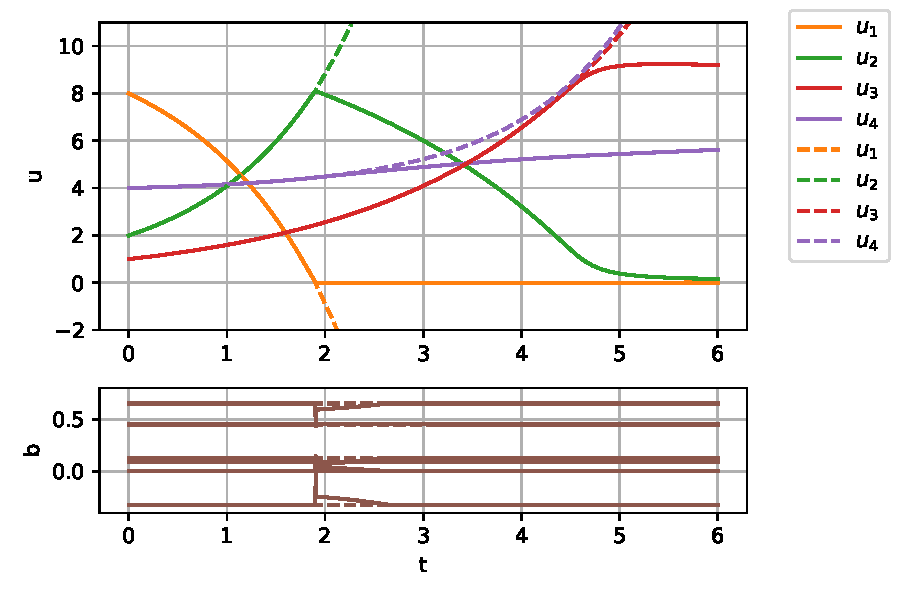
\includegraphics[width=0.75\textwidth]{plots/exampleI.pdf}
    \caption{Numerical approximation of the Reaction Problem from \cite{kopecz_comparison_2019}. Computed with ck5 and $\dt = 0.005$. The dashed lines are the reference (Note: Reference might be misleading here because real solution is different) solution without the adaption of the weights. The lower plot are the weights }
    \label{fig:exampleI}
\end{figure}

The used weights $b_1,\cdots,b_5$ are also plotted in Figure\,\ref{fig:exampleI}. 
The used weights are equal to the original weights for $t<1.905$. At $t=1.905$ the weights are first adapted to ensure the positivity of the solution. For $t>2.63$ the original set of weights lead to a positive solution. Because of this, the used weights equal the original weights again.


\section{Details (TODO: better title)}\label{sec:LP}

In the following section, it is explained how the approach can be written as a LP. 
For this we have to consider which weights to choose. 
Generally, any $b \in \R$ can be used. 
A first requirement would be that the new solution is positive.
We can further reduce this space by enforcing the order conditions. 
By incorporating the order conditions, the space of possible weights is limited to a subspace of $\R$. %(Note: not linear because 0 is not in subspace)
Finally, we have to give an objective function to get the optimal weights.


\subsection{Example II}\label{sec:example_lin}

(Note: The primary goal here is to put the idea of changing the b into perspective. We have shown the general idea and how it works, now we want to discuss on what it does in practice. At first, we state it is good to preserve the order... Get to the Example ... and show that there is more to it)


The main goal is to choose a $(A,b)$ in such a way that $u^{n+1}$ resembles the solution of the ODE $u(t_{n+1})$. 
A obvious objective is to use a $(A,b)$ with a high order, but this is not enough.
To get a better understanding for the method we consider the behavior of a simple problem.   

We take the linear, positivity preserving ODE from \cite{kopecz_unconditionally_2018} with $u = [u_1,u_2]^T$ with the initial conditions $u_0 = [1,0]^T$ and

\begin{equation}
u'(t) = L u(t) \qquad L = \left[\begin{matrix}- 5 & 1\\5 & -1\end{matrix}\right] 
\end{equation}
and and use the three Stage and third order SSP method (SSP33)
\begin{align}
\begin{array}{c|ccc}
0 &  &  & \\
1 & 1 &  & \\
\frac{1}{2} & \frac{1}{4} & \frac{1}{4} & \\
\hline
 & \frac{1}{6} & \frac{1}{6} & \frac{2}{3}\\
\end{array}
\end{align}
The Matrix $L$ has the eigenvalues $\lambda_1 = -6,\lambda_2=0$. The real stability interval of the SSP33 method includes $[-2.5,0]$. The method is absolut stable for this problem with $\dt = \frac{1}{3}$
The stage derivatives are
\begin{equation}
f(y_1)=\left[\begin{matrix}-5\\5\end{matrix}\right]\qquad f(y_2)=\left[\begin{matrix}5\\-5\end{matrix}\right]\qquad f(y_3)=\left[\begin{matrix}-5\\5\end{matrix}\right]\end{equation}
The values of the next step using the standard weights is
\begin{equation}
u_n=\left[\begin{matrix}- \frac{1}{9}\\\frac{10}{9}\end{matrix}\right]
\end{equation}
The new solution contains negative values. 
Therefor we want to adapt the weights to ensure positifity. 
All weights that comply with the order Condition for the first and second order can be expressed as
\begin{equation}
\tilde b=\left[\begin{matrix}\frac{1}{6}\\\frac{1}{6}\\\frac{2}{3}\end{matrix}\right]+\alpha \left[\begin{matrix}\frac{1}{2}\\\frac{1}{2}\\-1\end{matrix}\right]
\end{equation}
With this we have one degree of freedom for the choice of the weights. This is done by the parameter $\alpha$.
If the general expression for the weights is inserted in \eqref{eq:Combination} the general solution is 
\begin{equation}
u^{1} = u^0 + \dt  \left[f(y_1),f(y_2),f(y_3)\right] b =
\left[\begin{matrix}- \frac{1}{9}\\\frac{10}{9}\end{matrix}\right] +\alpha \left[\begin{matrix}\frac{5}{3}\\- \frac{5}{3}\end{matrix}\right]
\end{equation}
By changing the parameter $\alpha$ the weights $b$ and the solution is altered.
With a suitable choice of $\alpha \in \left[\frac{1}{15},\frac{2}{3}\right]$ any $u$ that complies with mass conservation and positivity can be reached. 
By adding additional constraints on the weights the choice of $\alpha$ can be narrowed down. 
An objective function is also needed to make the choice unique. This should be designed in a way to prefer weights that are close to the original weights.


%This gives raise to the question whether the new solution is reasonable.
%This also poses the problem on developing a system that can decide if the new solution is has to be rejected. 





\subsection{Order Conditions}\label{sec:OrderCond}

The order conditions for a RKM are a set of Equations depending on $A$, $c$ and $b$. In these Equations $b$ only appears linearly \cite{hairer_solving_1993}.
If $A$ and $c$ are already known, the order conditions for the Order $p$ are a linear equations system and can be written as $Q b = r$. 

The vector $b \in \R^s$ contains the weights and $Q$ is an $g \times s$ matrix, where $g$ is the number of order conditions. The vector $r$ contains the right hand side of the order conditions.

If the $A$ of a preexisting RK-method is used, there is at least one solution for the linear equation system.
In order to get an optimization problem, the equation system has to be underdetermined.
This implies that $\mathrm{rank}(Q) < s$. 
Because the quadrature conditions are linearly independent, there are at least $p$ independent vectors in $Q$. This leads to the condition $p < s$.
This implies that the number of stages has to be higher than the wanted order.



\subsection{Ways to formulate the Optimization Problem}

There are two possible ways to write down the adaptation of the weights. The first way is to directly adapt the original weights $b$ by adding a correction $\Delta b$ that ensures positivity.
This is the easiest way to adapt the weights. An advantageous property is that the step size can be reduced after calculating the stage values by using the dense output order conditions.  
The direct adaption is explained in more detail in section\,\ref{sec:direct}.

The second way to formulate a LP is to choose weights as a convex combination of a set of weights. This is more useful if some embedded methods with certain properties are known. 
The convex combination also shows more predictable behavior because the resulting $u^{n+1}_b$ is also a convex combination of the solutions $u^{n+1}_{b_a},u^{n+1}_{b_b},\cdots$ 
This is explained in more detail in section\,\ref{sec:convex}

Both approaches are illustrated in figure\,\ref{fig:b_space}.


\begin{figure}
    \centering
    \begin{subfigure}[b]{0.45\textwidth}
        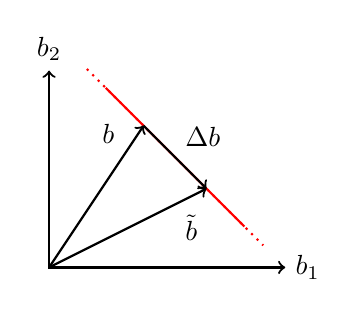
\begin{tikzpicture}
    % Draw axes
	\coordinate (borig) at (1.2,1.8);
    \coordinate (b) at (2,1);
	\coordinate (db) at ($(b)-(borig)$);

    \draw [<->,thick] (0,2.5) node (yaxis) [above] {$b_2$}
        |- (3,0) node (xaxis) [right] {$b_1$};


%Add subspace 
	\draw[thick,red,dotted] ($-0.9*(db)+(borig)$) -- ($0.9*(db)+(b)$);
	\draw[thick,red] ($-0.6*(db)+(borig)$) -- ($0.6*(db)+(b)$);
	
	\draw[thick,->] (borig) -- node[anchor=south west ,pos = 0.5] {$\Delta b$} (b);
	\draw[thick,->] (0,0) -- node[anchor=south east,pos = 0.8] {$b$} (borig);
    \draw[thick,->] (0,0) -- node[anchor=north west,pos = 0.8] {$\tilde{b}$} (b);

\end{tikzpicture}
        \caption{Direct Adaptation}
        \label{fig:b_direct}
    \end{subfigure}
    \begin{subfigure}[b]{0.45\textwidth}
        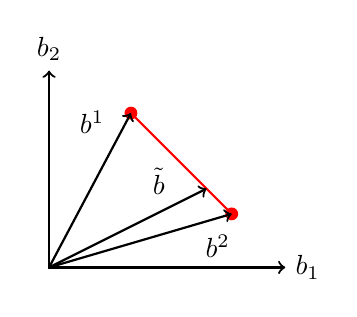
\begin{tikzpicture}
    % Draw axes

	\coordinate (bo) at (1.2,1.8);
    \coordinate (b) at (2,1);
    \coordinate (db) at ($(b)-(bo)$);
    \coordinate (b1) at ($0.4*(db)+(b)$);
    \coordinate (b0) at ($-0.2*(db)+(bo)$);;

    \draw [<->,thick] (0,2.5) node (yaxis) [above] {$b_2$}
        |- (3,0) node (xaxis) [right] {$b_1$};

%\draw[thick,red,*-*] (b0) -- (b1);
   \node[circle,inner sep=1.5pt,draw,fill,red] (A) at (b0) {};
   \node[circle,inner sep=1.5pt,draw,fill,red] (B) at (b1) {};
   \draw[thick,red,-] (b0) -- (b1);


	\draw[thick,->] (0,0) -- node[anchor=south east,pos = 0.8] {$b^1$} (b0);
    \draw[thick,->] (0,0) -- node[anchor=south east,pos = 0.8] {$\tilde{b}$} (b);
    \draw[thick,->] (0,0) -- node[anchor=north west,pos = 0.8] {$b^2$} (b1);





\end{tikzpicture}

        \caption{Convex Combination}
        \label{fig:b_convex}
    \end{subfigure}
    \caption{Graphical representation of the two different approaches to adapt the weights}\label{fig:b_space}
\end{figure}

\subsection{Direct Adaptation}\label{sec:direct}

When directly adapting the weights new weights that complies with the order conditions is chosen.   
The weights $\tilde{b} = b + \Delta b$ consist of the weights of the original method $b$ and an adaption $\Delta b$. The adaption is $\Delta b \in \mathrm{ker}(Q)$. 
This is drawn in Figure\,\ref{fig:b_direct}. The red line represents the subspace of weights that satisfie the order conditions. Both $b$ and $\tilde{b}$ are in this subspace. 
The LP can be expressed as


\LPblock{
\begin{subequations}
\begin{align}
u^{n+1}&=u^n+\dt F \tilde{b} \geq 0 \label{eq:direct_pos}\\
Q\tilde{b} &=r \label{eq:direct_Order} \\
\min_{\tilde b}&( ||\tilde{b} -b ||_1) \label{eq:direct_obj} 
\end{align}
\end{subequations}
}


\subsubsection{Constraints}
The Direct Adaptation approach leads to two sets of constraints on $b$.
The first set of constraints is the positivity \eqref{eq:direct_pos}.
The second set of constraints are the order conditions in \eqref{eq:direct_Order}.

\subsubsection{Objective Function}
A reasonable property of the objective function would be that for the LP only constrained by the order condition the optimal solution is $\tilde{b} = b$. 
This can be achieved by $argmin(f_{optim}(\tilde{b})) = b$. 
In practice, this also means that there is no need to solve the optimization problem if no constraints are violated because the solution of this problem is already known. This is advantageous for performance reasons.
Large values of b can lead to numerical problems. Because $\sum_{i  = 1}^s b_i = 1$, an increase of $||b||$ leads to a combination of negative and positive values. Because the computation is done with a finite precision (and usually in floating point) large $||b||$ can lead to numerical difficulties.    
By changing the weights the stability function is altered. 
For these reasons $||\tilde{b}-b||$ seems like a good choice. The 1-Norm can be implemented in a  LP using slack variables. We choose \eqref{eq:direct_obj}
as objective function.



\subsubsection{Adaption of Timestep using the dense output formual}

If the original step $\dt$ was too large and there is no suitable set of weights, the LP is infeasible. In this case we would like to calculate $u^{n+\theta}$ using the stage values instead of rejecting the step. For this the time step is reduced after calculation the stage values. This can be done using the order conditions for dense output. These can be found in \cite{hairer_solving_1993}.
We introduce $\theta \in (0,1]$. The new step taken has the length $\theta \dt$ whereas $\dt$ is the time step used when calculating the stage values.
To calculate a reduced step the order conditions have to be adapted and a new $b(\theta)$ for the objective function has to be generated. 
When adapting the Order Condition to a new $\theta$ the Order Condition Matrix $Q$ stays unchanged whereas the right hand side $r(\theta)$ depends on $\theta$.

The dependency of $r(\theta)$ is nonlinear. This means that the maximum $\theta$ with suitable weights cannot be calculated by solving a LP. This means that different $\theta$ have to be tested. 
%(Note: we could include some algorithm to search for it)

\subsection{Convex combination of existing methods}\label{sec:convex}
For some test problems (e.g. the Heat Equation solved with an implicit method of higher order), large changes occur, even though a norm of $\Delta b$ is used as an objective function. A numerical example is given in Section\,\ref{sec:Numeric_Results}.
It is known that the backward Euler method lead to a positive solution for any $\dt$ \cite{hundsdorfer_numerical_2003}. The backward Euler is still only first Order but shows more exact results than a method of higher Order that is distorted by the adaption of the weights, at least at some steps. 
A possible method to fix this is to generate the new b based on a convex combination of embedded methods. 
The new weights are defined as 
\begin{equation}\label{eq:b_convex_def}
\tilde{b} = \sum_i^d g_i b_i = Bg
\end{equation}
where $B=\left[b_1,\cdots,b_d \right]$ is a matrix containing the embedded methods.  
The LP is defined as
\LPblock{
\begin{subequations}
\begin{align}
 u^{n+1}&=u^n+\dt K B g \geq 0 \label{eq:Convex_pos}  \\
 0 \leq g_i &\leq 1  \forall {i \in \{1, \cdots d \}} \quad \sum_{i=1}^d g_i = 1 \label{eq:Convex_cvx} \\
 \min_{g} &\left(\sum_i^d w_i g_i \right) \label{eq:Convex_obj}
\end{align}
\end{subequations}
}

\subsubsection{Constraints}
At first a set of embedded methods of the RKM $b_1,\cdots,b_d$ is needed. 
If all the used weights complie with the order conditions the new method is also of the same Order.
This is straightforward using
$$ Q b = Q (\chi b_{\alpha} + (1-\chi) b_{\beta}) = \chi Q  b_{\alpha} + (1-\chi) Q b_{\beta} = \chi r + (1-\chi) r = r$$
$b_{\alpha}$ and $b_{\beta}$ are the methods that are combined to $b$ using the parameter $\chi$. The Matrix $Q$ and the vector $r$ are the order conditions as defined in Section\,\ref{sec:OrderCond}.
To ensure that \eqref{eq:b_convex_def} yields to a convex combination the constraints \eqref{eq:Convex_cvx} are enforced for the parameters $g_1,\cdots,g_d$.
The positivity constraint changes to \eqref{eq:Convex_pos}

\subsubsection{Objective Function}

As an objective function \eqref{eq:Convex_obj}
is used.  The $w_1,\cdots,w_d$ are weighting factors that determine which is the preferred $b_i$ to use.

Because the optimal solution of the unconstrained problem has to be the original weights the weight corresponding to $b$ should be the smallest $w$. This weight is simply set to $w_{b} = 0$. For the other weights $w_i = \frac{1}{\mathrm{Order} \{b_i\}}$ is used. This prefers embeded methods of higher order.

\subsubsection{Construction of Embedded Methods}

As a first order method, the weights that corresponds to a series of backward Euler steps are added. These are known to yield a positive result for any step size.
It is also possible to add embedded methods of higher order.
An important property of the embedded methods is that they should show the desired stability characteristics. 

A reduction of the step size using the order conditions for dense output would also be possible. For this a set of embedded methods $b_1(\theta),\cdots,b_d(\theta)$ has to be constructed. This was not the aim of this research.

(Note: Doing dense Output here is a bit complicated, but it would not help ensure positivity only (maybe) increase exactness.  is it worth exploring this or is it better to just leave this open for further research it may be also interesting regardless the study of positivity)
 
\section{TODO: Title} \label{sec:integration}

In the previous sections an algorithm for choosing positifity preserving weights $\tilde{b}$ has been presented. 
In the following section, it is explained how this Algorithm can be integrated into the framework of existing solvers.

\subsection{Choice of Baseline Method}
An important property for the used baseline method is the existence of embedded methods and the degrees of freedom for the b.
As noted in Section\,\ref{sec:OrderCond} the number of stages has to be higher than the order. 
Another important property is the number of degrees of freedom for the choice of the new weights. 
These can be calculated using $s-\mathrm{rank}(Q)$.%$\mathrm{dim}(\mathrm{ker}(Q))$.
The number of degrees of freedom for different methods are shown in table\,\ref{table:DOF_exp} for explicit methods and in table\,\ref{table:DOF_imp} for implicit methods.

\begin{table}[h!]
\centering    %Generated below============ 
\begin{tabular}{|l |c c c c c c |} 
 \hline 
Order &1&2&3&4&5&6 \\ 
 \hline Classical RK4&3&2&0&0& - & -  \\ 
 SSPRK(10,4)&9&8&6&4& - & -  \\ 
 Cash-Karp RK5(4)6&5&4&2&1&0& -  \\ 
 Dormand-Prince RK5(4)7&6&5&3&1&0& -  \\ 
 \hline 
 \end{tabular}
 \caption{Degrees of Freedom for Choice of the weights} %Generated above============ 
 \label{table:DOF_exp}
 \end{table}
 
 \begin{table}[h!]
\centering   %Generated below============ 
 \begin{tabular}{|l |c c c c c c |} 
 \hline 
Order &1&2&3&4&5&6 \\ 
 \hline Implicit Euler&0& - & - & - & - & -  \\ 
 Im-Euler 2&2&1& - & - & - & -  \\ 
 Im-Euler 3&5&4&2& - & - & -  \\ 
 Im-Euler 4&9&8&6&3& - & -  \\ 
 \hline 
 \end{tabular}
 \caption{Degrees of Freedom for Choice of the weights} %Generated above============ 
 \label{table:DOF_imp}
 \end{table}


For all methods with the number of stages equal to the order of the method, there are no degrees of freedom without reducing the order. 
If the classical RK4 method is used the Order has to be reduced more because the RK4 method does not have embedded methods of order 3.
Contrary to this methods with $s > p$ have degrees of freedom even without reducing the order. 

Another important property is the stability region. The adaption of the weights does solve issues with stabilitz when used with a too big $\dt$. Therefore the RK-method has to be stable for large $\dt$.

%(Note: up to this point I do not understand why some methods perform better than other. We only see it occur depending on the Problem-RKM combination)

A third property is the existence of a positive solution. This corresponds to the question if there is an embedded first order method that ensures positivity. This is particularly interesting for implicit methods, because the $\dt$ is not limited by the stability. 
If we have an embedded first Order Method we can ensure that there is always a positive solution, which might be of first Order. 

\subsection{Error detection and Approximation}
When changing the weights the solution $u^{n+1}$ is changed. 
By incorporating the order conditions for a certain order the space of possible weights that can be chosen is limited to a linear Subspace. 
Now it is important to know if the new solution $u^{n+1}$ still resembles the solution of the ODE $u(t_{n+1})$. 
This can be seen in example in section\,\ref{sec:example_lin}.
By a suitable choice of $\alpha \in [\frac{1}{6},\frac{7}{30}]$ any $u$ that complies with mass conservation and positifity can be reached. 

This gives rise to the question whether the new solution is reasonable.
This also poses the problem on developing a system that can decide if the new solution is has to be rejected. 
 
\subsubsection{Error Detection and Appproximation}
For this approach it is difficult to give some mathematically rigorous statement regarding the convergence of the method, because it only applies if the error of the original method causes the solution to get negative. This can only happen if the truncation error is large enough. This requires $\dt \gg 0$ where lower coefficients of the Taylor series are no longer sufficient to approximate the behavior. 
One could say that the main idea of the adaption of the weights alters the error in a certain way, so that the numerical solution gets 'better' in the sense that it leads to positive solutions. 
The local error of a RKM $e(\dt) =u(t_0 + \dt) - u^1$ can be expressed using the Taylor series of the RKM and the Taylor series of the exact solution. % Hairer I P134

\begin{align}\label{eq:Taylor_sol_ref}
u(t_0 + \dt) &= u(t_0) + u'(t_0) \dt + \frac{u''(t_0)}{2} \dt^2 + \cdots + \frac{u^{(p)}(t_0)}{p!} \dt^p + \frac{u^{(p+1)}(t_0)}{(p+1)!} \dt^{p+1} + \cdots \\
u^{n+1} &= u(t_0)  + v_1 \dt + \frac{v_2}{2} \dt^2 + \cdots + \frac{v_p}{p!} \dt^p + \frac{v_{p+1}}{(p+1)!} \dt^{p+1} + \cdots 
\end{align}

The derivatives of $u(t)$ can be solely expressed with the partial derivatives of the RHS $f(t,u)$, whereas the coefficients $v_1,v_2,\cdots$ also depend on the RKM. 
In this case the RKM is fixed apart from the weights. 
Therefore $v_1,v_2,\cdots$ are functions of $b$.
Because the the weights are chosen to ensure the Order Conditions the coefficients $v_1,\cdots,v_p$ are fixed and equal the according derivatives. 
The only remaining degrees of freedom are the coefficients $v_{p+1},v_{p+2},\cdots$.
These can be adapted by changing the weights.

%The main way to ensure that the RKM with adapted b converges to the correct solution is to ensure that the weights approaches $b_{orig}$ for $\dt \to 0$. For this the weights it is already known that the numeric solution converges to the exact solution.  
%This is made sure by the property of the Objective function that 
%\begin{equation}
%\mathrm{argmin}(f_{optim}(b)) = b_{orig}
%\end{equation}
This approximation is not very useful for real applications. 
To approximate the error of a new step we propose following approximation of the local error:

\begin{align}
err = |u(t^n)-u^n| &= |u(t^n) - (u^n_{b_{orig}+\dt K(b-b_{orig})})| \\
 &\leq \underbrace{|u(t^n)-u^n_{b_{orig}}|}_{\approx err_T}+\underbrace{|\dt K(b-b_{orig})|}_{= err_{adapt}} \label{eq:Err}
\end{align}

After adapting the weights the approximation error is checked. If $|\dt K(b-b_{orig})|$ is larger than the tolerance the weights are rejected. 

%\subsubsection{Steppsize Control}
%An important part of an RKM method is the ability to approximate the error of the solution to use it to control the step size. 
The truncation error $|u(t^n)-u^n_{b_{orig}}|$ is usually approximated with an standard error estimator $err_T = | u^{n}_{b_{orig}} - u^{n}_{\hat{b}} |$.
Both errors are added to get an approximation of the total error $err = err_T + err_{adapt}$. %The parameter $w_a \leq 1$ is used to account for the fact that the real error is smaller than $err = err_T +err_{adapt}$. The factor also improves the stability of the step size control because $err_{adapt}$ is not as smooth as $err_T$, especially if negative values only occur for a small number of steps.
%If the LP was infeasible and no weights were found the $err_{approx}$ is set to a custom value. This value should be chosen sufficiently large to ensure that the next step take is smaller, but still not too large to keep the step size control stable.
This type of error estimation is easy to implement because it can be easily incorporated in an existing step size control and takes advantage of the standard error approximation.

%To make sure that the new adapted solution is still reasonable we measure the deviation from the Original method. In the worst case the errors add up. (todo: here some math formula... (We know that cannot be the case because we already know that we will reduce the error for the quantity we will make positive, still we can use it as a upper bound.))

\subsection{Stability Region}

By adapting the $b$ the used RK Method is changed. This also alters the stability function and therefore changes the region of absolute stability. 
It depends on the solved problem, the RKM and the used $\dt$ by how many steps the stability function is altered. For problems where only a small number of steps are affected a bigger change in the stability function would be acceptable. For problems which require an adaptation of the weights for every step one needs to make sure that the resulting method is stable.


\begin{figure}
     \centering
     \begin{subfigure}[b]{0.45\textwidth}
         \centering
         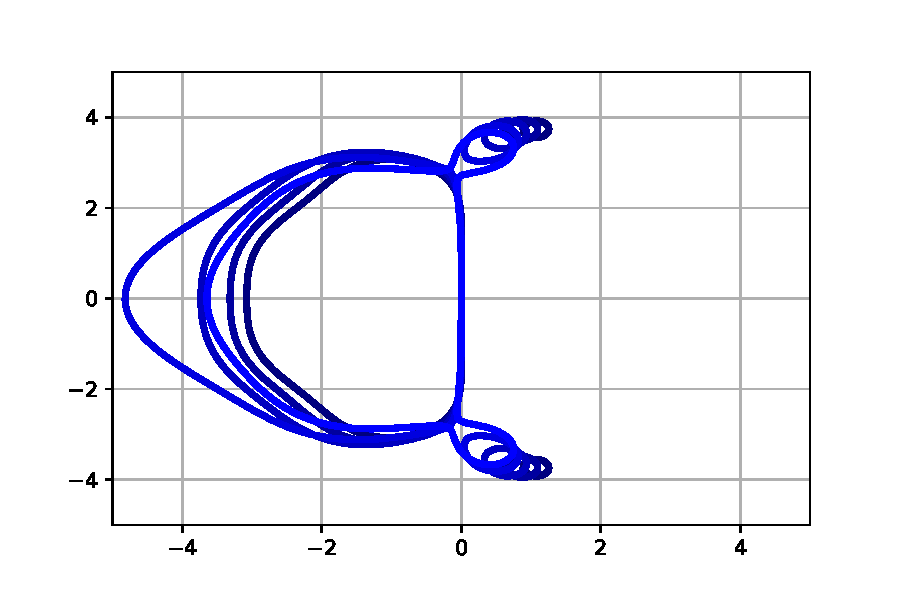
\includegraphics[width=\textwidth]{plots/stab_ck5.pdf}
         \caption{Cash-Karp 5}
         \label{fig:stab_ck5}
     \end{subfigure}
     \hfill
     \begin{subfigure}[b]{0.45\textwidth}
         \centering
         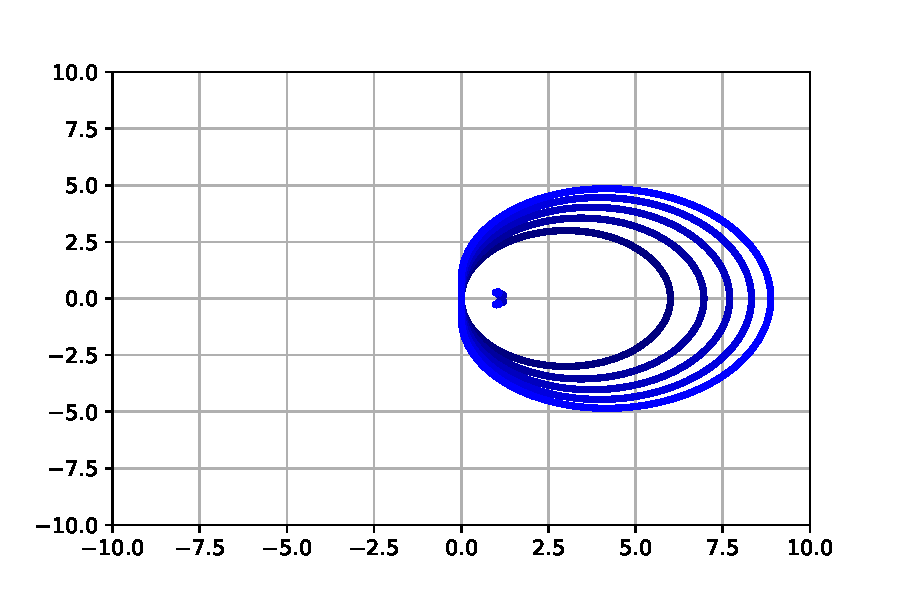
\includegraphics[width=\textwidth]{plots/stab_ex3.pdf}
         \caption{Implicit Extrapolation 3}
         \label{fig:stab_ex3}
     \end{subfigure}
        \caption{Change of stability region for direct adaptation(a) and for convex combination(b) (TODO: legend, axis, description in text)}
        \label{fig:stab}
\end{figure}



\paragraph*{Version 1} $ $\\

The stability function is defined as 
\begin{equation}\label{eq:stab_func}
R(z) = 1 + zb^T(I - zA)^{-1}e
\end{equation}
We can define a function $P(z)$
\begin{equation}
P(z) = R(z)-1 = z b^T (I - zA)^{-1} e
\end{equation}
These rational functions are $\in \mathcal{L}^\infty$. (Note: for all explicit methods this is always true, for implicit methods we have to exclude the poles $\{z | \det(I - zA) = 0\}$ or  $\{z | \det(I - zA) > \epsilon \}$ )
We define $\mathcal{P}$ as all $P(z)$ for the class of $RKM_A$. 
This is a vector space.
Proof:
\begin{multline}
\alpha P_a(z) + \gamma P_c(z) =  \alpha z a^T (I - zA)^{-1} + \gamma z c^T (I - zA)^{-1} =\\
z (\alpha a+ \gamma c)^T (I - zA)^{-1} = P_{\alpha a + \gamma c}(z) \in \mathcal{P}
\end{multline}

The $P(z)$ is a linear combination of the rational functions
\begin{subequations}
\begin{align}
p_1(z) &= z e_1^T (I - zA)^{-1}\\
\vdots \\
p_s(z) &= z e_s^T (I - zA)^{-1}
\end{align}
\end{subequations}
whereas $e_1,\cdots,e_s$ is the standard basis of $\R^s$.
These span $\mathcal{P}$. If $p_{e_1}(z),\cdots,p_{e_s}(z)$ are linearly independent $p_{e_1}(z),\cdots,p_{e_s}(z)$ are a basis of $\mathcal{P}$.

With this results the stability function $R_b(z)$ of any RKM in $RKM_{(A)}$ can be calculated with 
\begin{equation}
R_b(z) = 1 + P_b(z) = 1 + \sum_{j = 1}^s b_s p_{e_1}
\end{equation}




\paragraph*{Version 2} $ $\\
The stability function is defined as a function $\CN \to \CN$ with 
\begin{equation}\label{eq:stab_func}
R(z) = 1 + zb^T(I - zA)^{-1}e
\end{equation}
We can add $b$ as a second parameter and get a function $\CN \times \R^s \to \CN$ with
\begin{equation}\label{eq:stab_func}
R(z,b) = 1 + zb^T(I - zA)^{-1}e
\end{equation}
The stability function is a linear function in the weights.

\paragraph*{Version 3} $ $\\
(Ignore this topic, because the following sections also can work without it)

%(Todo: It is not straightforward if there are no pole zero cancellations in the stability function. For explicit methods, the stability function is a polynomial o degree $\leq s$ (Hundsdorfer). Pole zero cancellations cannot happen for these. For implicit functions that are A-stable the poles have to be in the right halve plane. Here is starts to get interesting. Because the A-Stability of one method with a certain $A$ is not a sufficient condition that there are no Poles for all RKM with this A-Matrix. But it is possible (or easy) to prove that if $a_{ii} > 0 \forall i = 1,\cdots , s$ then there are only poles in the right halve plane where they do not matter for the further considerations.)


\subsubsection{Stability of convex combination}
If the new weights are chosen as a convex combination of weights it is easy to prove properties of the stability region.
The stability function $R_{\chi b_a + (1-\chi) b_b}(z)$ of a convex combination can be calculated by the weighted sum of the stability functions $R_{b_a}(z)$ and $R_{b_b}(z)$

Proof:
\begin{multline}
R_{\chi b_a + (1-\chi) b_b}(z) = R(z) = 1 + (\chi b_a + (1-\chi) b_b)^Tz(I - zA)^{-1}e \\
= \chi + (1-\chi) + \chi b_a ^Tz(I - zA)^{-1}e + (1-\chi) b_b^Tz(I - zA)^{-1}e \\
= \chi R_{b_a}(z) + (1-\chi) R_{b_b}(z)
\end{multline}

The resulting region of absolute stability is at least the intersection of the regions of absolute stability of the methods that define the convex combination. This also means that if all the used embedded methods used to construct the new weights are A-Stable, the resulting method is also A-Stable.

We want to show that the convex combination of two methods is absolutely stable at the points where both original methods were absolutely stable.
This can be formulated as $(|R_{b_a}(z)|  < 1) (|R_{b_b}(z)| < 1) \Rightarrow |R_{\chi b_a +(1- \chi) b_b}(z)| < 1$ with $\chi \in [0,1]$.


\begin{multline}
|R_{\chi b_a +(1-\chi) b_b}(z)| = |\chi R_{b_a}(z) + (1-\chi) R_{b_a}(z)| \leq |\chi R_{b_a}(z)| + |(1-\chi) R_{b_a}(z)|\\
 =| \chi| \underbrace{|R_{b_a}(z)|}_{<1} + |(1-\chi)| \underbrace{|R_{b_a}(z)|}_{<1} < \chi + (1-\chi)= 1
\end{multline}



\subsubsection{Stability of  Direct Adaptation}
If the weights is adapted directly there is no such proof.
A useful property of the resulting stability region is that it is similar to the stability region of the baseline method. 
(Note: is it possible (or needed at all) to give some statement like: If the stability regions of the RKM used for multiple steps are similar, then the overall method is stable for the intersection of the stability regions.)

For most methods, a small change of the weights does not alter the stability function dramatically.
(TODO: I am missing a piece here from ‘the derivative is finite’ to ‘is similar’)

We would like to calculate the derivative of the border in respect to a change of the weights. 

The stability function depending on the weights is expressed. 
When adapting the weights we cannot change them independently but only in ways that comply with the order conditions.
$m$ is the number of dimensions of the Kernel of the Order Condition $m = \mathrm{dim}\{\mathrm{Ker} (Q) \}$
The $b_1,\cdots,b_m$  are the Basis vectors of $\mathrm{Ker} (Q)$. With a coordinate transformation we get the coordinate vector $\hat{b}$ with the Matrix $B = [b_1,\cdots,b_m]$ and $b = B \hat{b}$.

The general stability function of all embedded RKM that satisfy the Order Conditions $Q$ is given by 

\begin{equation}\label{eq:gen_stabilityf}
R(\hat{b},z) = 1 +  (b_{orig} +B \hat{b})^T z(I - zA)^{-1}
\end{equation}
The border is defined by the implicit function 
\begin{equation}\label{eq:border}
|R(\hat{b},u+iv)|^2 -1 = 0
\end{equation}
This function can be viewed either as $\R^m \times  \CN \rightarrow \R$ or $\R^m \times  \R^2 \rightarrow \R$.
We are only concerned with the expansion or contraction. Because of this we are only interested in the change perpendicular to the border of the stability region. 

For a point $z_0= u_0 +i v_0 $ 
with $ |R(w,z_0)|^2 -1 = 0 $ the gradient of
 $|R(w,u,v)|^2$ is calculated. 
If the gradient does not vanish at $z = z_0$ \eqref{eq:border} can be transformed in a function $\R^m \times \R \rightarrow \R$ depending on $\hat{b}$ and a single variable $a$ by setting $z = z_0 + n a$. The complex number $n$ denotes the normal vector $\vec{n} = \frac{\nabla |R(\hat{b},u,v))|^2}{\left| \nabla |R(\hat{b},u,v))|^2 \right|}$ of the border of the stability region written in complex notation. This defines the function $a(\hat{b})$ with $|R(\hat{b},z_0 + n a(\hat{b}))|^2 -1 = 0$. 
This implies that this approach is only applicable if the gradient does not vanish on the border of the stability function. This is not true in general but for the most common RKM. 
The derivative $\frac{\mathrm d}{\mathrm d \hat{b}} (a(\hat{b}))$ can be calculated using the implicit function theorem. The defining function is 
\begin{equation}\label{eq:f(w,a)}
f: \R^m \times \R \rightarrow \R f(\hat{b},a) = |R(\hat{b},z_0 + n a)|^2 -1 
\end{equation}
If explicit methods are used this function is known to be continuously differentiable because it can be written as a polynomial of $\hat{b},u$ and $v$. This is a necessary condition for the use of the Implicit function theorem. 
It is also known by definition, that for the point $b = b_{orig}$ and $z = z_0$ the equation $ |R(\hat{b},z_0)|^2 -1 = 0 $ is satisfied.
For simplicity only the formulas for the derivative at the value $b = b_{orig}$ are given. This corresponds to $\hat{b} = 0$.
The wanted derivative is given by 

\begin{equation}
 \frac{\partial a}{\partial \hat{b}_j} (w) =
 - \left[ \frac{\partial f}{\partial a} (\hat{b},a(\hat{b}))  \right] ^{-1} 
   \left[ \frac{\partial f}{\partial \hat{b}_j}(\hat{b},a(\hat{b})) \right]
\end{equation}
as long as $\frac{\partial f}{\partial a} \neq 0$ on the border of the region of absolute stability. This is true in most cases as it has been discussed above.

The derivative of \eqref{eq:f(w,a)} in respect to $a$ evaluated at $\hat{b}=0$ can be calculated using the directional derivative
\begin{align*}
 \frac{\partial f}{\partial a} \Big|_{\hat{b}=0} =& 
 \frac{\partial f}{\partial a} (\hat{b},a(\hat{b})) \Big|_{\hat{b}=0} = 
 \nabla |R(\hat{b},a(\hat{b})|^2 \vec{n} \Big|_{\hat{b}=0} \\
=& \left| \nabla|R(0,z_0)|^2 \right| = \left| \nabla|R_{b_{orig}}(z_0)|^2 \right|
\end{align*} 

The derivative in respect to $\hat{b}_j$ is 
$ \frac{\partial f}{\partial \hat{b}_j}(\hat{b},a(\hat{b})) \Big|_{\hat{b}=0}$.
This simplifies to 
\begin{multline}\label{eq:derivative_to_b}
 \frac{\partial f}{\partial \hat{b}_j}(\hat{b},a(\hat{b})) \Big|_{\hat{b}=0} = 
 \frac{\partial }{\partial \hat{b}}(R(\hat{b},z)R(\hat{b},z^*)) \\
 = (B\hat{b}_j)^T (I-zA)^{-1} R_{b_{orig}}(z^*) + (B\hat{b}_j)^T (I-z^*A)^{-1} R_{b_{orig}}(z)
\end{multline}
using the fact that $z_0$ is on the border of the stability region.
The derivative $(B\hat{b})^T (I-zA)^{-1} R_{b_{orig}}(z^*) (B\hat{b})^T (I-z^*A)^{-1} R_{b_{orig}}(z)$ is known to be finite for explicit methods, because it is a polynomial and $|z_0| < \infty$
The same process can be done for all points on the border of the stability region. 
As long as $\nabla|R(\hat{b},u+iv)|^2 \neq 0 \forall \hat{b} < \epsilon  \forall z$ the derivative $\frac{\partial a}{\partial \hat{b}_j} (\hat{b})$ is finite. This means that a small change of the weights only leads to a small change of the stability region.


\section{Implementation aspects of the Algorithm}\label{sec:imple}

TODO: Discuss in this section aspects that are needed for implementation (and improve the usability) but do not concern the mathematical idea of the approach.

\subsection{Positivity}


For the further discussion, we are concerned with a system of $m$ coupled ODEs. 
In this setup $u \in \R^m$.
Systems of ODEs with a high number of dimensions can appear when solving a PDE with the method of lines.

To ensure that the solution is positive 

\begin{equation}
 u_i^{n+1} \geq 0   \quad   \forall {i \in \{1, \cdots,m \}}  
\end{equation}
has to be fulfilled.
This infers $m$ positivity constraints to the optimization problem. These can be written as

\begin{equation}
u_i + \dt \sum_{j=0}^s F_{i,j}  b_j \geq 0 \quad \forall {i \in \{1, \cdots,m \}}  
\end{equation}

This causes unnecessarily many inequality constraints on the LP. To simplify the problem, one wants to reduce the number of positivity constraints by ignoring it for ODEs where there is no issue with positivity.
The new positivity constraints can be formulated as
\begin{equation}
u_i + \dt \sum_{j=0}^s F_{i,j}  b_j  \geq 0 \quad   \forall {i \in h \subseteq \{1,\cdots,m \}} 
\end{equation}
For this a set $h$ that includes all indecies $i \in \{1,\cdots,m \}$ that are needed for determining the weights has to be chosen.

A reasonable approach is to set $h_0 = \{ i \in \{1,\cdots,m \} |  u_i^{n+1}  < 0 \}$. 
After the new weights and $u^{n+1}$ is computed using $h_0$, the algorithm has to check if the positivity of the other values $u_i | i \notin h_0 \subseteq \{1,\cdots,m \}$ is still met. 
If the condition is not met a new set $h_{a+1} = \{ i \in \{1,\cdots,m \}|  u_i^{n+1}  < 0 \} \cup h_{a}$ using the new $u^{n+1}$ is generated and the LP is solved again. This process is repeated until a solution is found that leads to a $u^{n+1} \geq 0$. The choice of $h_{a+1}$ based on the $h_{a}$ ensures that the algorithm cannot get stuck in a loop. In the worst case $h_a$ is growing very slowly until $h_a = \{1,\cdots,m \}$. 
This worst case did not occur when runing the testproblems. 
%(Note: A approach on this would be to make a educated guess which indices could get a problem with positivity. A possible estimate would be $\frac{u_i^{n+1}}{max(K_{(i,0)}, \cdots ,K_{(i,0)})} $ )

When enforcing a maximum value the number of constraints can be reduced using the same technique. When nforcing both maximum and minimum values two separate sets of active constraints $k_{min}$ and $k_{max}$ are used. The set $k_{max}$ denotes the active maximum constraints and the set $k_{min}$ denotes the active minimum constraints. 
In this case it is important to update these sets simultaneously.  

\subsection{Implemention}
(Todo: Maybe a flowchart and a description on how we stitch everything together.) 

At fist the stagevaules and stagedeerivatives are calculated.
After this $u^{n+1}$ is computed using the original weights. If the positivity is not violated, this solution is used to update the solution. 
If $u^{n+1}$ contains negative values, the weights are adapted using the following algorithm.
For this different orders are tried, stariting with the highest order that has degrees of Freedom for $\tilde{b}$. 
At first the Order Conditions are constructed. On these a LP-Solver is invoiced. If the LP is infeasible the algorithm immediately reduces the order. If the LP is feasible we test if the solution is acceptable. At first it is tested weather the new $u^{n+1}$ indeed complies with the constraints. This is necessary because sometimes the used LP-solvers incorrectly identify the problem as feasible. %(Note: because of the chosen objective function it cannot be unbounded) 
Afterwards the adaption error is calculated using \eqref{eq:Err}. If the error is bigger than a set maximum error the $\tilde{b}$ is also rejected.
If the new set of weights is requected in one of the tests the order is reduced.
As soon as the algorithm finds suitable weights these are used to update the solution.
If all acceptable orders are tried and no weights were found the step hast to be requected.
If the reduction of stepsize is used this process is done first for $\theta = 1$. If no weights were found, the process is repeated for a smaler $\theta$. 



\section{Results of experiments}\label{sec:Numeric_Results}

(Note: Is here a good place to give a note on where supplementary code can be found?)

(Note: Should we discuss which solver is used. Probably it is not worth using space for some plot etc. on this... Maybe a short note?)

\subsection{Applicable Problems}\label{sec:app_problem}
The approach can be used with ODE systems $u' = f(t,u)$ that ensure  $u(t) \geq 0 \forall t \forall {  u_0 \geq 0}$ 
A sufficient condition is  
\begin{equation}
u_i=0 \Rightarrow f_i(t,u_1,\cdots,u_i,\cdots,u_n) \geq 0  \forall {u_c \geq 0} \forall {t}
\end{equation}
For problems where the exact solution is positive for certain $u_0$ but positivity is not preserved for all $u_0 \geq 0$ tests did not show promising results. Additionaly it is not certain if the computed solutions would be reasonable.


\subsection{Explicit methods}
First we want to test the adaptive RKM used with explicit methods. 
When used with explicit methods the cost of solving the LP significant because the computation of the stagevalues only requires $s$ evaluations of the RHS.
For most of the linear test problems tried the explicit methods jield to positive results. 
When increasing the stepsize issues with stability occur before getting negative values. 
An example therefore the ODE in in Section\,\ref{sec:example_lin}.
Some nonlinear RHS may require very small timesteps to preserve positifity. 
For these adapting the weights could be a possible way to solve them.
An Exmample is the Reaction equation solved in Section\,\ref{sec:example_reac}.
The positivity of stagevaulues is not esured, therefore the right had side has to be defined for negative values. If this is not the case, the right hand side has to be defined for negative values.
%All the following testproblems did not nead this modification.

As test problem the PDE
\begin{equation}
\frac{\partial u}{\partial t} = -a \frac{\partial u}{\partial z} - K (u)
\end{equation}
is simulated with the method of lines on the domain $x = [0,1]$ with $N =100$ points. The Problem consists of a Advection part and an Exponential decay. At $x=0$ a inflow boundary with $u(0,t)=1$ is used. The initial condition is $u(x,0)=0$
As semidiscretization an upwinding scheme is used. This leads to positivity preserving ODE
\begin{equation}
\frac{\mathrm d}{\mathrm d t} u_i = \frac{a}{\Delta x} \left( u_{i-1} - u_i \right) - K u_{i-1}
\end{equation}
The parameters are set to $a=1$ and $K=1$.
We use the Dorman-Prince 5 RKM and adapt the weights using the direct adaptation.
In Figure\,\ref{fig:sol_AdDe} the results for $\Delta t = 0.02$ are plottet for different timesteps. We can see that the solution approaches a exponential function with $t \rightarrow \infty$.
In Figure\,\ref{fig:weights_AdDe} the used weights are plotted. For $t\leq 0.6$ the weights are altered. For $t > 0.6$ the original weights lead to a positive solution.
\begin{figure}
\centering
\begin{subfigure}[b]{0.45\textwidth}
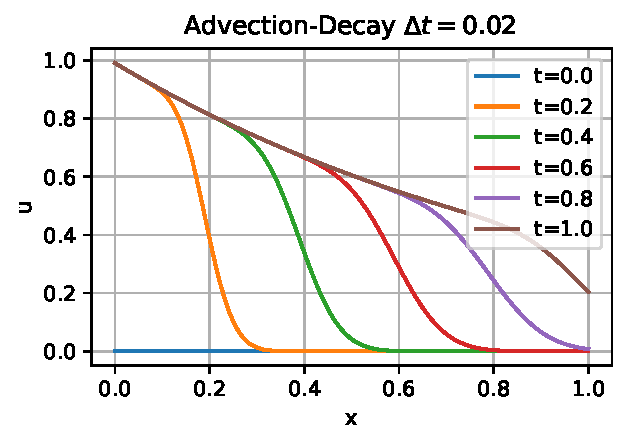
\includegraphics[width=1\textwidth]{plots/Advection_Decay.pdf}
\caption{Solution of Advection Decay Problem}
\label{fig:sol_AdDe}
\end{subfigure}
\\
\begin{subfigure}[b]{0.45\textwidth}
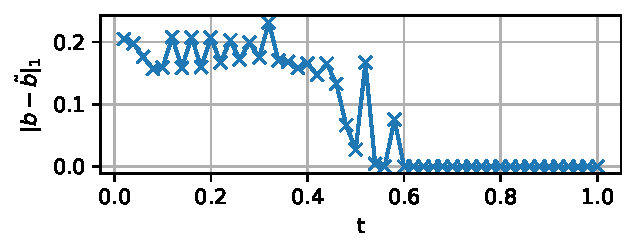
\includegraphics[width=1\textwidth]{plots/b_Advection_Decay.pdf}\\
\caption{Weights used for Advecion Decay Problem}
\label{fig:weights_AdDe}
\end{subfigure}
\end{figure}


Next different timesteps are used.
For $\dt \leq 0.0082$ the unaltered method leads to positive solutions. For a larger $\dt$ the original method leads to negative values and the weights are altered. For $\dt >0.016$ the dp5 is no longer stable.
For the ODE the refernce solution can be computed using the matrix exponential. 
In Figure\,\ref{fig:conv_expl} the convergence for $t=0.5$ is plotted for the altered and unaltered method.

\begin{figure}[h]
\centering
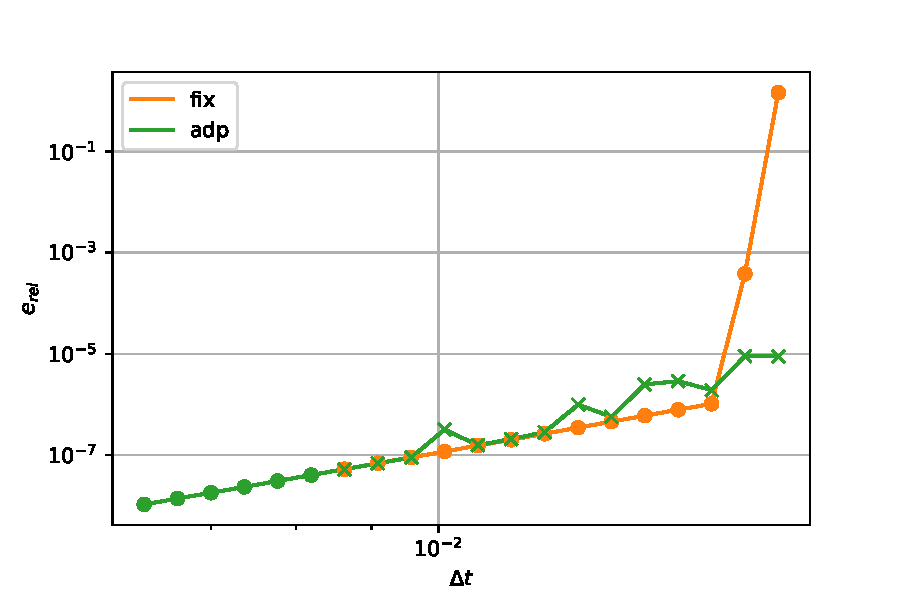
\includegraphics[scale=0.75]{plots/conv_adde.pdf}
\caption{Convergence adapted dp5}
\label{fig:conv_expl}
\end{figure}

The unaltered method has the order $p=5$. 
The values marked with an cross denote the numerical experiments that required an adaption of the weights. 
Even though the order is reduced most errors are still close to the error of the unaltered method.

\subsection{Implicit methods}
Implicit methods seem like an advantageous choice for a couple of reasons.
At first the cost of solving the LP is relativeley small compared to the cost of solving the stageequations.
Second the timestep is not limited by the stability of the method.
Therefore it is possible to use larger timesteps, that are more likely to lead to negative values.
A very interesting calss of methods are the implicit extraploation methods. These are Diagonaly implict and $p < s$. This means that they allow for changes of the weights without a reduction of the order.
Also all stegevalues are computed using the BE method. This means that all intermedaite stages are nonnegative. 
Also a embeded BE euler step is included. This ensures that an positive solution always exists, even if it is of first order. 

We test the adaptive RKM on the diffusion equation 
\begin{equation}
\frac{\partial }{\partial t} = D \frac{\partial^2}{\partial x^2}
\end{equation}
with homogeneous Dirichlet boundary conditions on the domain $x = [-0.5,0.5]$ with $N=100$ points. The equation is semidiscreticed using the 3-point-scheme
\begin{equation}
\frac{\mathrm d}{\mathrm d t} u_i = \frac{d}{\Delta x^2} \left( u_{i-1} - 2u_i + u_{i+1} \right)
\end{equation}
As initial condition $u^0 = (0,\cdots,0,1,0,\cdots,0)^T$ is used. The diffusion coefficient is$D=1$
The ODE is solved using the implicit EX3 method. 
For large (Note: better word for 'not small enough') $\dt$ the method computes negative values for $u^1$.
These can be corrected by adapting the weights. 
The solutions are computed using the direct adaptation and convex combination for $\dt = \num{1e-3}$
The results for the direct adaptation are plotted in Figure\,\ref{fig:sol_Diff_a}. The used weights are plotted in Figure\,\ref{fig:weights_Diff_a}.
The original solution for the first step are negative. Therefore the weights have to be changed.
If we take a look at the solution after the first timestep at $t=0.001$ we can see that $x=0$ the solution is samler than the solution at the surrounding points. 
This is not physical. 
The next timesteps lead to physical solutions again.
To prevent this glitch from happening we choose the weights based on a convex combiantion.
A first order embedded method is added. The solution is shown in Figure\,\ref{fig:sol_Diff_c} and the weights are plotted in Figure\,\ref{fig:weights_Diff_c}.
The weights for the first step are altered again.
The weights obtained by the convex combination are different from the weighst obtained
by taking the direct adaptation.
The solution for $t=0.001$ computed with the convex combination is physical.
For both approaches the remaining steps can be computed with the standard weights.

\begin{figure}
\centering
\begin{subfigure}[b]{0.45\textwidth}
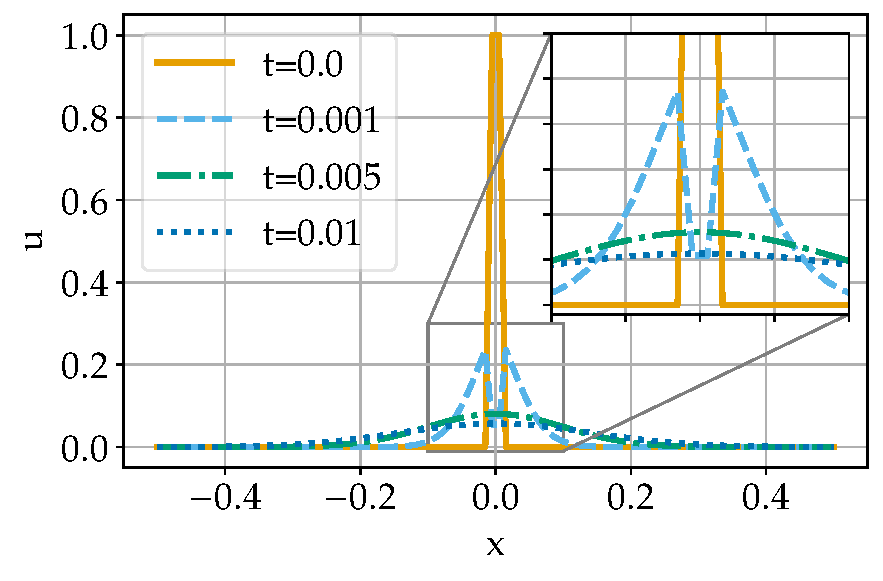
\includegraphics[width=1\textwidth]{plots/Diff_Direct.pdf}\\
\caption{Solution of Diffusion for direct adaptation}
\label{fig:sol_Diff_a}
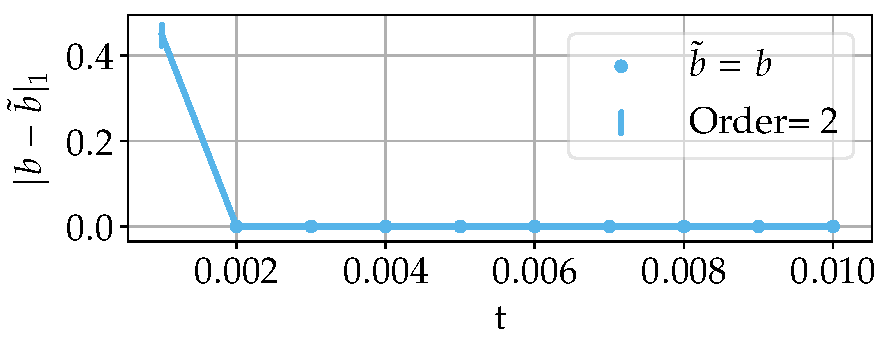
\includegraphics[width=1\textwidth]{plots/b_Diff_Direct.pdf}\\
\caption{Weights used for direct adaptation}
\label{fig:weights_Diff_a}
\end{subfigure}
\begin{subfigure}[b]{0.45\textwidth}
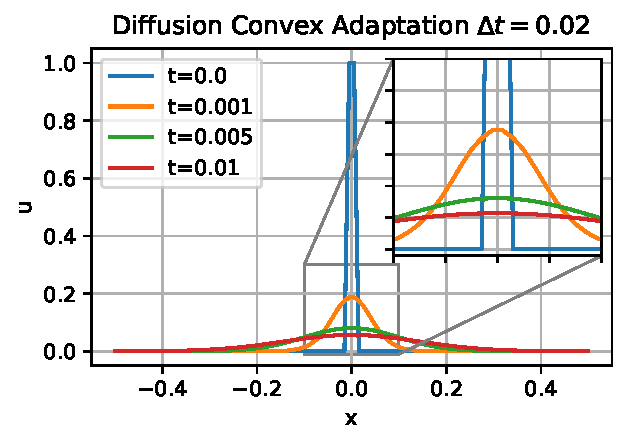
\includegraphics[width=1\textwidth]{plots/Diff_Convex.pdf}\\
\caption{Solution of Diffusion for convex combiantion}
\label{fig:sol_Diff_c}
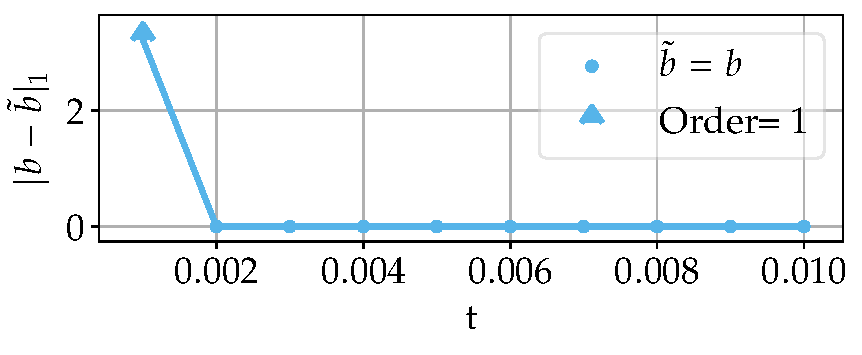
\includegraphics[width=1\textwidth]{plots/b_Diff_Convex.pdf}\\
\caption{Weights used for convex combination}
\label{fig:weights_Diff_c}
\end{subfigure}
\end{figure}


In figure\,\ref{fig:conv_impl} the convergence is shown for the unalteres EX3 method, that potentially leads to negative vaules, the adaptive method with direct adaptation (EX3a) and the adapted method using convex combiantions (EX3c). 
Also the BE method is plotted. It is only of 1st order but preserves positivity for all $\dt$.
For $\dt < \num{3e-5} $ the standard weights yield to a positive result. For larger $\dt$ the weights have to be adapted to ensure positivity.
The EX3a shows similar convergence properties than the original method.
This can be expected, because the adapted method is still of 3rd order.
The EX3c has larger errors than the EX3a but leads to physical solutions for all time-steps. 
This is no supprise because the adapted RKM used for the first step is only of 1st order.
But the adaptive method still outperformes the BE, even when acocunting for the higher cost per step.

\begin{figure}[h]
\centering
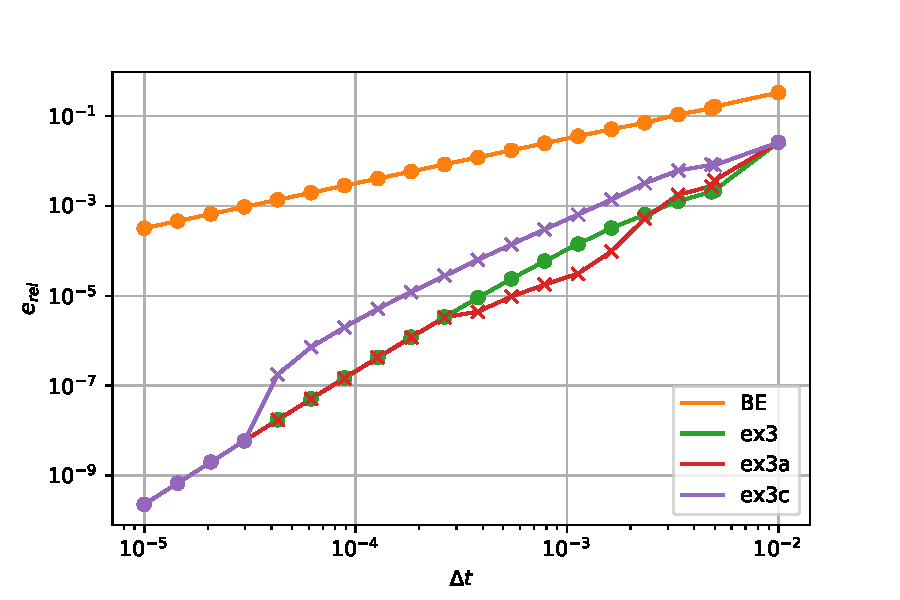
\includegraphics[scale=0.75]{plots/conv_heat.pdf}
\caption{Convergence adapted ex3}
\label{fig:conv_impl}
\end{figure}


\subsection{Stepsize control}

Next we test the adaptive RKM on a more compelx problem. 
For this we consider the advection-diffusion-production-destruction systems form \citep{kopecz_comparison_2019}. The system is defined by
\begin{subequations}
\label{eq:ADR}
\begin{align}
\frac{\partial u_1}{\partial t} &=-a \frac{\partial u_1}{\partial x} + d\frac{\partial^2 u_1}{\partial x ^2} + 0.01u_2 + 0.01 u_3 +0.003u_4 - \frac{u_1 u_2}{0.01+u_1} \\ 
\frac{\partial u_2}{\partial t} &=-a \frac{\partial u_2}{\partial x} + d\frac{\partial^2 u_2}{\partial x ^2}\frac{u_1u_2}{0.01+u_1} -0.01 u_2-0.5(1-\exp(-1.21 u_2^2)) u_3 -0.05 u_2 \\ 
\frac{\partial u_3}{\partial t} &=-a \frac{\partial u_3}{\partial x} + d\frac{\partial^2 u_3}{\partial x ^2} + 0.5(1-\exp(-1.21u_2^2)) u_3 - 0.01 u_3 -0.02 u_3 \\ 
\frac{\partial u_4}{\partial t} &=-a \frac{\partial u_4}{\partial x} + d\frac{\partial^2 u_4}{\partial x ^2} + 0.05 u_2 + 0.02 u_3 + 0.003u_4 
\end{align}
\end{subequations}

With the parameters $    a=\num{1e-2} $ and $ d=\num{1e-6}$.
The PDE is simulated on the doamin $x = [0,1]$ with $N=100$ points. Periodic boundarie conditions are used.
The advecion part is semidiscreticed using a first order upwind sheme and the diffusion part is semidiscreticed using a 3-poin-scheme. This leads to a positivity preserving system of ODEs. 
The computation is done using the EX3 method with direct adaptation.
As stepsize control a PI-Control from\,\cite{hairer_solving_1996} is used. The Error was estimatet using \eqref{eq:Err}. The Tolerance was set to $Tol = 0.01$. 
The final time is $t_{end} = 50$.
The simulation required 264 steps. Of these 72 required a adaptation of the weights.
The solutions for $t=9,t=18,t=27$ and $t=50$ are plotted in Figure\,\ref{fig:Sol_ADP}.
In Figure\,\ref{fig:sol_ADP18} it can be seen that the reaction occurs in a small interfaces.
Outside of this regions quantities are close to $0$. Therefore it is very likely that negative values orrur in the numerical approxiamtion.
In Figure\,\ref{fig:sol_ADP27} it can be seen that at $T=27$ the two reaction interfaces merged. Afterwards the reaction stops and the behavoir is mainly controlled by the advection and diffusion part.

In Figure\,\ref{fig:Stats_ADP} different vaules are plottet. 
In the first subplot the stepsize is plotted. For $t<25$ the timesteps are small. After $t = 30$ the the stepsize increases, because the solution only evovlves slowly afterwards.
In the second subplot the $min(u_1,u_2,u_3,u_4)$ is plotted for all timesteps that initaily lead to negative values. This value is computet before and after adapting the weights. 
We can see that relativley large negative values occured at some timesteps.
After the adaption of the weights all values are cloes to $0$. Therfor the adaption of weights succesfully preserved positifity.
In the third subplot the approxiamted truncation error $err_T$ and the adaption errro $err_{adapt}$ are plotted.
We can see that the adaption error is of a similar magnitude as the truncation error. Therefore the totoal error of the method is not increased drastically. 
In the last subplots the weights are ploted. 
We can see that the cahnges to the weights are only very small. The adapted RKM is still very close to the original RKM.


\begin{figure}
    \centering
    \begin{subfigure}[b]{0.49\textwidth}
        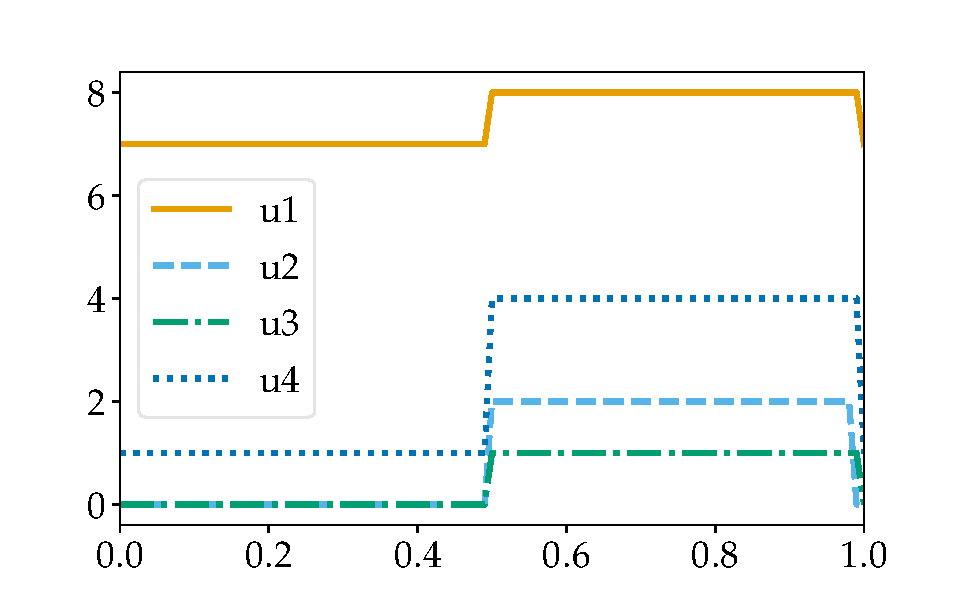
\includegraphics[width=\textwidth]{plots/ADP_sol_00.pdf}
        \caption{$t=0$}
        \label{fig:sol_ADP00}
    \end{subfigure}
    \begin{subfigure}[b]{0.49\textwidth}
        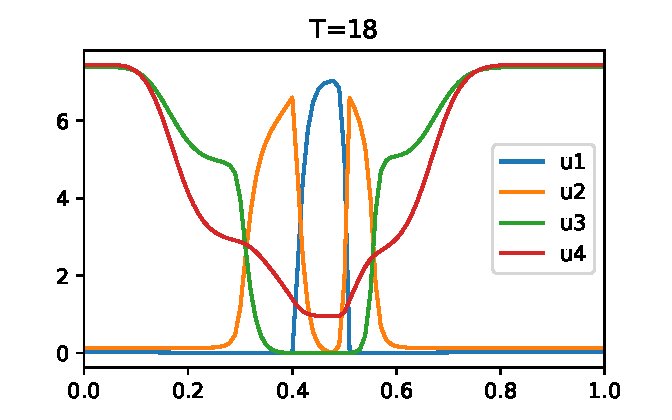
\includegraphics[width=\textwidth]{plots/ADP_sol_18.pdf}
        \caption{$t=$}
        \label{fig:sol_ADP18}
    \end{subfigure}
    
    \begin{subfigure}[b]{0.49\textwidth}
        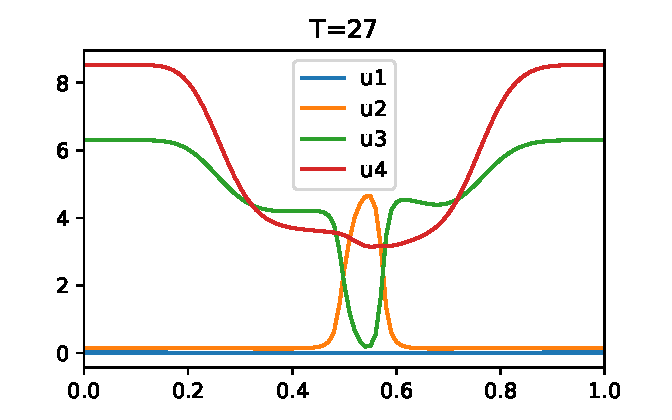
\includegraphics[width=\textwidth]{plots/ADP_sol_27.pdf}
        \caption{$t=$}
        \label{fig:sol_ADP27}
    \end{subfigure}
	\begin{subfigure}[b]{0.49\textwidth}
        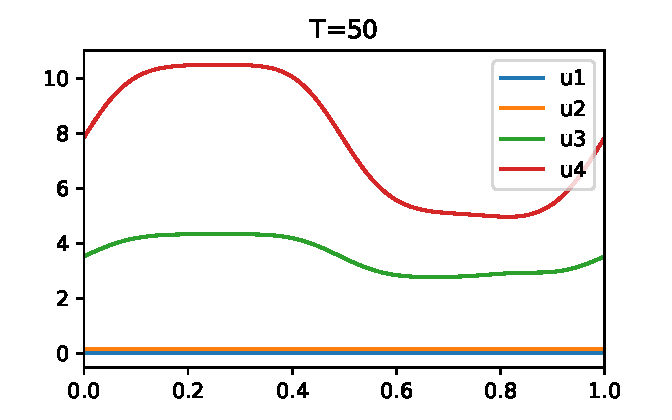
\includegraphics[width=\textwidth]{plots/ADP_sol_50.pdf}
        \caption{$t=$}
        \label{fig:sol_ADP50}
    \end{subfigure}

    \caption{Solution of Advection-Diffusion-Reaction Problems at different times}\label{fig:Sol_ADP}
\end{figure}

\begin{figure}
\centering
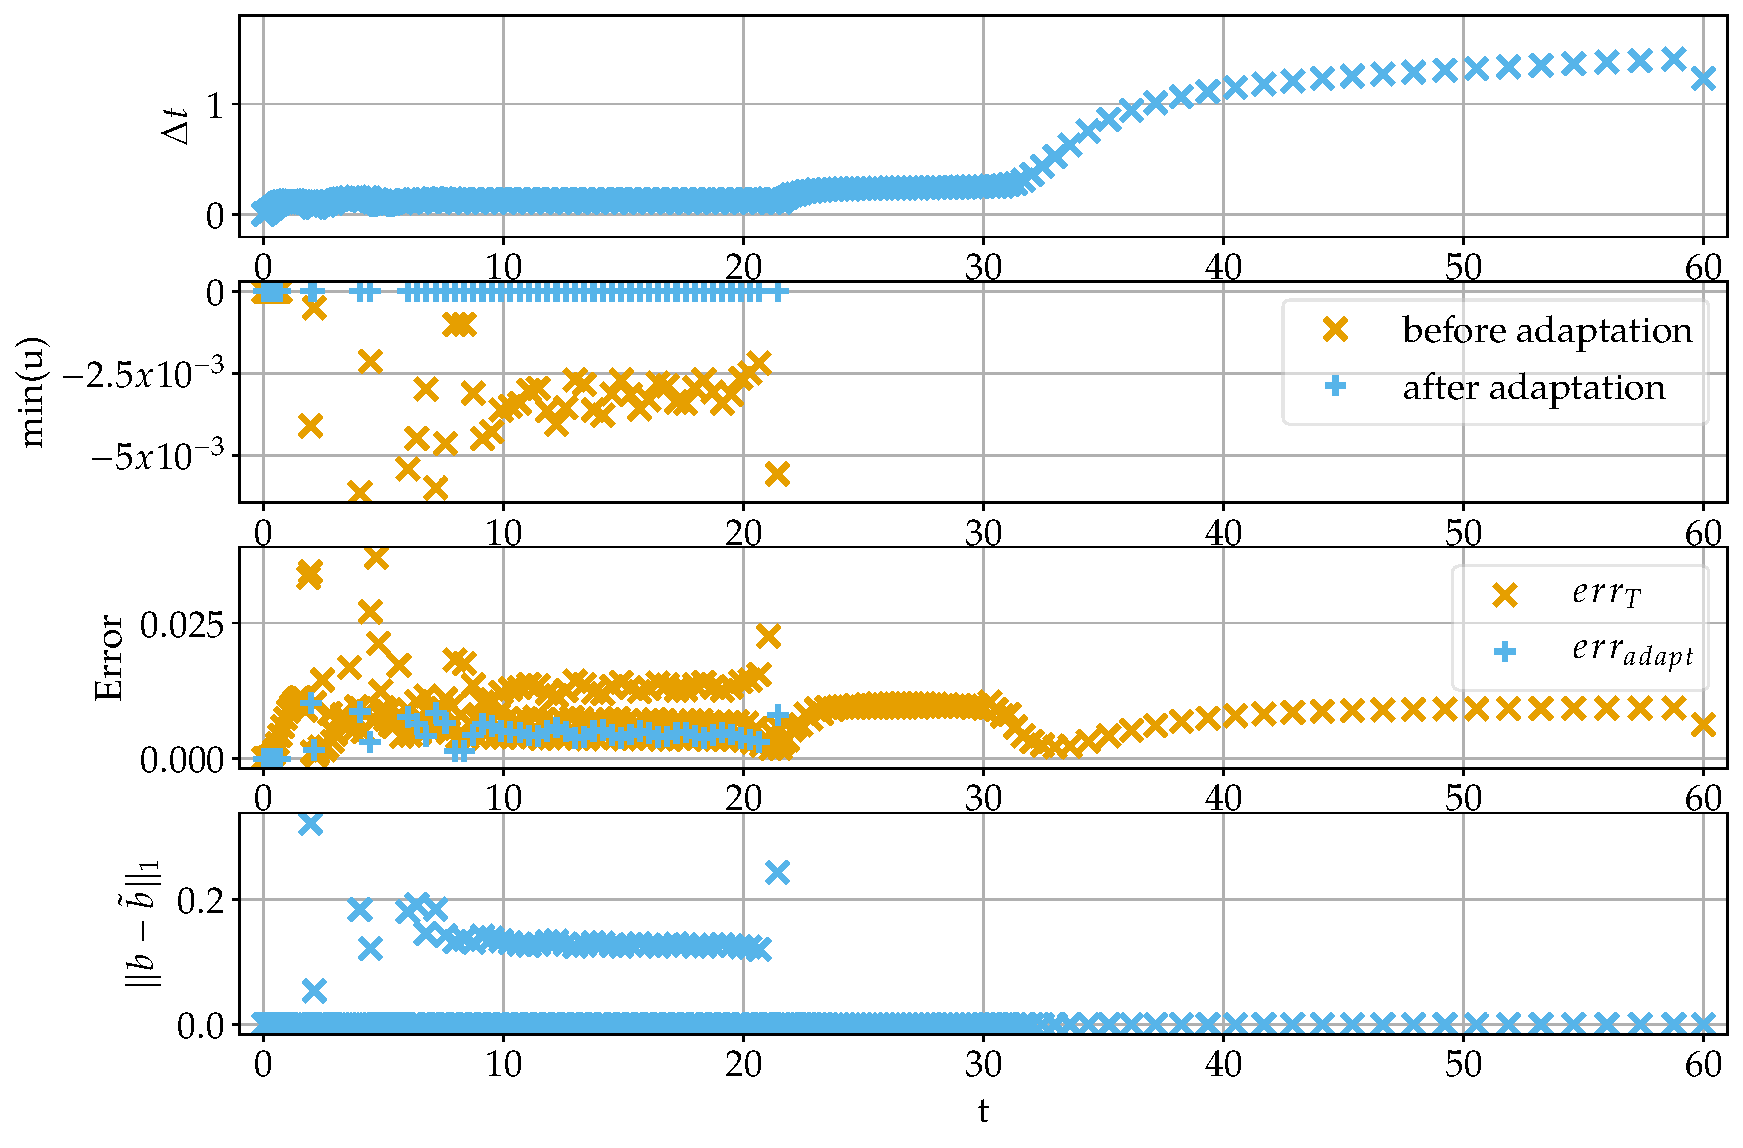
\includegraphics[width=0.85\textwidth]{plots/ADP_stepsize,b.pdf}
\caption{Different statistics of computation of ADPD-Problem}
\label{fig:Stats_ADP}
\end{figure}


\section{Conclusion} \label{sec:conclusion}
It is possible to adapt the weights to enforce positivity for RKMs that are not positifity preserving.
A main limitation is that the resulting Order has to be lower than the number of stages. 
An error approximation for this method was given. 
The region of absolute stability is altered by changing the weights. This effect can be predicted or controlled.
Used with explicit methods the positivity for some test problmes could be recovered. 
Because the time steps is limited by the stability it is only useful for a small interval of time steps.
The adaptive method mainly interesting for diagonally implicit methods. 
The times teps here are not limited by stability.
Also the cost of solving the LP is not crucial factor. 
If the negative values occurring are not to large, which can be expected for most computations, adapting the weights is a potential way to fix these.

%also if exactnes is not the limiting factor but positivity 



\printbibliography


\end{document}
